\documentclass[14pt,a4paper,report]{report}
\usepackage[a4paper, mag=1000, left=2.5cm, right=1cm, top=2cm, bottom=2cm, headsep=0.7cm, footskip=1cm]{geometry}
\usepackage[utf8]{inputenc}
\usepackage[english,russian]{babel}
\usepackage{indentfirst}
\usepackage[dvipsnames]{xcolor}
\usepackage[colorlinks]{hyperref}
\usepackage{listings} 
\usepackage{fancyhdr}
\usepackage{caption}
\usepackage{amsmath}
\usepackage{latexsym}
\usepackage{graphicx}
\usepackage{amsmath}
\usepackage{booktabs}
\usepackage{array}
\hypersetup{
	colorlinks = true,
	linkcolor  = black
}

\usepackage{titlesec}
\titleformat{\chapter}
{\Large\bfseries} % format
{}                % label
{0pt}             % sep
{\huge}           % before-code


\DeclareCaptionFont{white}{\color{white}} 

% Listing description
\usepackage{listings} 
\DeclareCaptionFormat{listing}{\colorbox{gray}{\parbox{\textwidth}{#1#2#3}}}
\captionsetup[lstlisting]{format=listing,labelfont=white,textfont=white}
\lstset{ 
	% Listing settings
	inputencoding = utf8,			
	extendedchars = \true, 
	keepspaces = true, 			  	 % Поддержка кириллицы и пробелов в комментариях
	language = C++,            	 	 % Язык программирования (для подсветки)
	basicstyle = \small\sffamily, 	 % Размер и начертание шрифта для подсветки кода
	numbers = left,               	 % Где поставить нумерацию строк (слева\справа)
	numberstyle = \tiny,          	 % Размер шрифта для номеров строк
	stepnumber = 1,               	 % Размер шага между двумя номерами строк
	numbersep = 5pt,              	 % Как далеко отстоят номера строк от подсвечиваемого кода
	backgroundcolor = \color{white}, % Цвет фона подсветки - используем \usepackage{color}
	showspaces = false,           	 % Показывать или нет пробелы специальными отступами
	showstringspaces = false,    	 % Показывать или нет пробелы в строках
	showtabs = false,           	 % Показывать или нет табуляцию в строках
	frame = single,              	 % Рисовать рамку вокруг кода
	tabsize = 2,                  	 % Размер табуляции по умолчанию равен 2 пробелам
	captionpos = t,             	 % Позиция заголовка вверху [t] или внизу [b] 
	breaklines = true,           	 % Автоматически переносить строки (да\нет)
	breakatwhitespace = false,   	 % Переносить строки только если есть пробел
	escapeinside = {\%*}{*)}      	 % Если нужно добавить комментарии в коде
}

\begin{document}

\def\contentsname{Содержание}

% Titlepage
\begin{titlepage}
	\begin{center}
		\textsc{Санкт-Петербургский Политехнический 
			Университет Петра Великого\\[5mm]
			Кафедра компьютерных систем и программных технологий}
		
		\vfill
		
		\textbf{Отчёт по лабораторной работе №5\\[3mm]
			Курс: «Администрирование компьютерных сетей»\\[3mm]
			Тема: «Создание макета сети в Cisco Packet Tracer»\\[35mm]
			}
	\end{center}
	
	\hfill
	\begin{minipage}{.5\textwidth}
		Выполнил студент:\\[2mm] 
		Ерниязов Тимур Ертлеуевич\\
		Группа: 13541/2\\[5mm]
		
		Проверил:\\[2mm] 
		Малышев Игорь Алексеевич
	\end{minipage}
	\vfill
	\begin{center}
		Санкт-Петербург\\ \the\year\ г.
	\end{center}
\end{titlepage}

% Contents
\tableofcontents
\clearpage

\chapter{Лабораторная работа №5}
\section{Цели работы}
\begin{enumerate}
\item Ознакомиться с Cisco Packet Tracer, и выполнить в нем:
\begin{itemize}
\item Построение компьютерной сети(из прошлых работ);
\item Настроить сервисы DNS, DHCP, TFTP;
\item Выполнить тестирование сети.
\end{itemize}
\end{enumerate}

\section{Построение компьютерной сети}
Средствами Cisco Packet Tracer была построена следующая схема:
\begin{figure}[h]
  \centering
  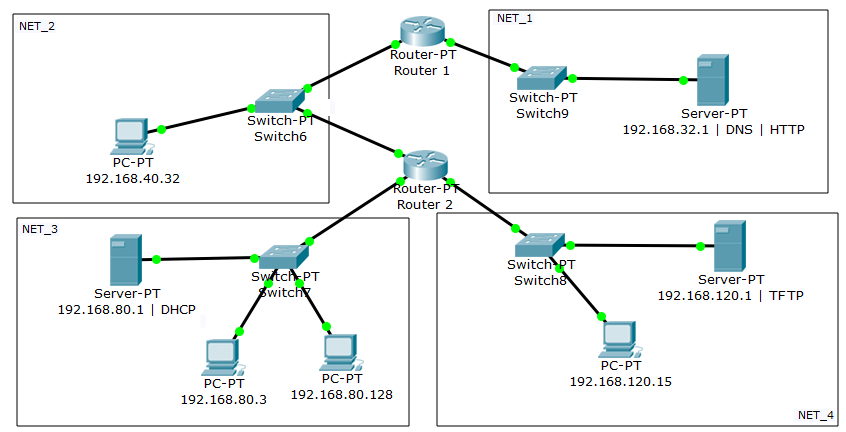
\includegraphics[width=\textwidth]{img/my_kks}
  \caption{Схема компьютерной сети}
\end{figure}
С помощью инструментов, были расставлены компьютеры, коммутаторы и роутеры типа \textbf{generic}, а также связаны между собой. По сравнению с работами в WMware, в данном случае:
\begin{itemize}
\item Вместо NetBSD и FreeBSD были использованы роутеры;
\item Вместо интернета выступает сервер с http страницой.
\end{itemize}


\begin{center}
\begin{tabular}{ c c c }
\textbf{Сегмент сети}&\textbf{Адрес узла}&\textbf{Описание}\\  
NET\_1&192.168.32.1&Сервер, с DNS и HTTP сервисами.\\ 
NET\_2&192.168.40.32&Компьютер, со статическим адресом.\\ 
NET\_3&192.168.80.1&Сервер, с DHCP сервисом.\\ 
NET\_3&192.168.80.3&Компьютер, адрес которого получен от DHCP сервера.\\ 
NET\_3&192.168.80.128&Компьютер, со статическим адресом.\\ 
NET\_4&192.168.120.1&Сервер, с TFTP сервисом.\\ 
NET\_4&192.168.120.15&Компьютер, со статическим адресом.\\ 
\end{tabular}
\end{center}

\subsection{Настройка адреса узла}
Для присвоения адреса какому-либо узлу, необходимо зайти в пункт \textbf{IP Configuration} и далее:
\begin{itemize}
\item Выбрать \textbf{DHCP}, если в сегменте сети имеется DHCP сервер;
\item Выбрать \textbf{Static}, если адрес предполагается статическим, и далее заполнить следующие поля:
\begin{itemize}
\item \textbf{IP Address};
\item \textbf{Subnet Mask};
\item \textbf{Default Gateway};
\item \textbf{DNS Server}.
\end{itemize}
\end{itemize}
После насктройки узла, для применения последних изменений рекомендуется перезагрузить его.

\subsection{Настройка сервисов}
Настройка DNS сервиса была произведена на узле с адресом 192.168.32.1. Для настройки необходимо выбрать, в меню настройки узла, пункт \textbf{DNS}, включить сервис и добавить новую запись. 

В данной работе была добавлена запись, со следующими параметрами:
\begin{itemize}
\item \textbf{name} - www.mypage.com
\item \textbf{address} - 192.168.32.1
\end{itemize}
То есть в данном случае, настраиваемый узел и является конечным узлом для данного доменного имени.

Также, для данного узла, был включен HTTP сервис, где уже имеется предварительно сгенерированная http-страница.\\\\
Настройка DHCP сервиса была произведена на узле с адресом 192.168.32.1. При которой были заполнены следующие поля:
\begin{itemize}
\item \textbf{Interface} - FastEthernet0;
\begin{itemize}
\item единственный интерфейс данного узла.
\end{itemize}
\item \textbf{Default Gateway} - 192.168.80.2;
\begin{itemize}
\item шлюзом по умолчанию выступает интерфейс роутера, подключенный к данной(NET\_3) подсети.
\end{itemize}
\item \textbf{DNS Server} - 192.168.32.1;
\begin{itemize}
\item предварительно настроенный DNS серверс из подсети NET\_1.
\end{itemize}
\item \textbf{Start IP Address} - 192.168.80.3;
\begin{itemize}
\item начала диапазона по выдаче IP-адресов.
\end{itemize}
\item \textbf{Subnet Mask} - 255.255.255.0;
\begin{itemize}
\item маска подсети.
\end{itemize}
\item \textbf{Maximun number of Users} - 100;
\begin{itemize}
\item максимальное количество пользователей.
\end{itemize}
\end{itemize}
Настройка TFTP сервиса была произведена на узле с адресом 192.168.120.15. Где его необходимо было включить, и для удобства удалить предварительно сгенерированные в нем файлы.


\subsection{Настройка роутеров}
В сети имеются два роутера(\textbf{Router 1} и \textbf{Router2}), которые выполняют функцию связующего звяна между подсетями.

\begin{center}
\begin{tabular}{ c c c }
\textbf{Роутер}&\textbf{Сеть}&\textbf{Адрес интерфейса}\\  
Router 1&NET\_1&192.168.32.128\\ 
Router 1&NET\_2&192.168.40.57\\ 
Router 2&NET\_2&192.168.40.2\\ 
Router 2&NET\_3&192.168.80.2\\ 
Router 2&NET\_2&192.168.120.2\\ 
\end{tabular}
\end{center}


Также, для корректной работы сети была добавлена маршрутизация. Для этого на Router 1, в настройках был выбран пункт \textbf{RIP Routing}, в который были добавлены следующие подсети:
\begin{itemize}
\item 192.168.32.0;
\item 192.168.40.0.
\end{itemize}
И для Router 2 соответственно:
\begin{itemize}
\item 192.168.40.0;
\item 192.168.80.0;
\item 192.168.120.0.
\end{itemize}

\section{Проверка}
\subsection{Проверка команды ping по адресу}
Откроем на узле 192.168.40.32(сеть NET\_2) утилиту \textbf{Command Prompt}, в которой введем команды \textbf{ipconfig} и \textbf{ping} в которой укажем адрес 192.168.120.15(сеть NET\_4).
\begin{lstlisting}[language={}]
C:\>ipconfig
FastEthernet0 Connection:(default port)
   Link-local IPv6 Address.........: FE80::2E0:A3FF:FEA3:7605
   IP Address......................: 192.168.40.32
   Subnet Mask.....................: 255.255.255.0
   Default Gateway.................: 192.168.40.2

C:\>ping 192.168.120.15
Pinging 192.168.120.15 with 32 bytes of data:
Reply from 192.168.120.15: bytes=32 time=1ms TTL=127
Reply from 192.168.120.15: bytes=32 time=1ms TTL=127
Reply from 192.168.120.15: bytes=32 time=1ms TTL=127
Reply from 192.168.120.15: bytes=32 time<1ms TTL=127

Ping statistics for 192.168.120.15:
    Packets: Sent = 4, Received = 4, Lost = 0 (0% loss),
Approximate round trip times in milli-seconds:
    Minimum = 0ms, Maximum = 1ms, Average = 0ms
\end{lstlisting}
Как видно из лога, команда пинг была успешна.

\subsection{Проверка команды ping по доменному имени}
Откроем на узле 192.168.80.3(сеть NET\_3) утилиту \textbf{Command Prompt}, в которой введем команды \textbf{ipconfig} и \textbf{ping} в которой укажем доменное имя \textbf{www.mypage.com}.
\begin{lstlisting}[language={}]
C:\>ipconfig
FastEthernet0 Connection:(default port)
   Link-local IPv6 Address.........: FE80::201:42FF:FE0B:D82B
   IP Address......................: 192.168.80.3
   Subnet Mask.....................: 255.255.255.0
   Default Gateway.................: 192.168.80.2

C:\>ping www.mypage.com
Pinging 192.168.32.1 with 32 bytes of data:
Reply from 192.168.32.1: bytes=32 time<1ms TTL=126
Reply from 192.168.32.1: bytes=32 time=10ms TTL=126
Reply from 192.168.32.1: bytes=32 time=11ms TTL=126
Reply from 192.168.32.1: bytes=32 time=13ms TTL=126

Ping statistics for 192.168.32.1:
    Packets: Sent = 4, Received = 4, Lost = 0 (0% loss),
Approximate round trip times in milli-seconds:
    Minimum = 0ms, Maximum = 13ms, Average = 8ms
\end{lstlisting}
Как видно из лога, доменное имя было преобразовано в адрес, по которому и была произведена команда ping.

\subsection{Проверка доступа к web странице}
На узле, с адресом 192.168.80.3(сеть NET\_3) была открыта утилита - браузер, в которой был введен адрес \textbf{www.mypage.com}.
\begin{figure}[h]
  \centering
  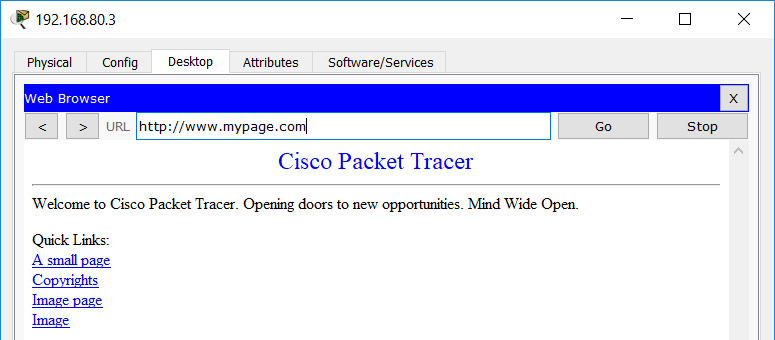
\includegraphics[width=.8\textwidth]{img/web}
  \caption{Web Browser}
\end{figure}
Как и ожидлось, страница была успешно загружена.

\subsection{Проверка TFTP}
На Router 2 была открыта консоль, в которой были выполнены следующие команды:
\begin{lstlisting}[language={}]
Router>enable
Router#show flash

System flash directory:
File  Length   Name/status
  3   5571584  pt1000-i-mz.122-28.bin
  2   28282    sigdef-category.xml
  1   227537   sigdef-default.xml
[5827403 bytes used, 58188981 available, 64016384 total]
63488K bytes of processor board System flash (Read/Write)

Router#copy flash tftp
Source filename []? pt1000-i-mz.122-28.bin
Address or name of remote host []? 192.168.120.1
Destination filename [pt1000-i-mz.122-28.bin]? temp.file

Writing pt1000-i-mz.122-28.bin...!!!!!!!!!!!!!!!!!!!!!!
[OK - 5571584 bytes]

5571584 bytes copied in 0.147 secs (8684467 bytes/sec)
\end{lstlisting}
Разберем действия:
\begin{enumerate}
\item Командой \textbf{enable} был совершен переход в привелегированный режим, можно заметить по символу решетки;
\item Командой \textbf{show flash} было выведено содержимое флеш-памяти, в данном случае это необходимо для тестовой загрузки по TFTP;
\item Командой \textbf{copy flash tftp} сообщаем о начале загрузке файла по tftp, где далее указывается файл(ы), tftp сервер для загрузки, а также новое имя файла(ов). 
\end{enumerate}
На TFTP сервере, в настройках TFTP появится выбранный ранее файл с указанным именем.



%На первичном сервере вводим команду \textbf{cat /etc/log/syslog}
%\begin{lstlisting}[language={}]
%...
%... zone example.com/IN: loaded serial 1
%... zone 40.168.192.in-addr.arpa/IN: loaded serial 1
%... zone 255.in-addr.arpa/IN: loaded serial 1
%... zone localhost/IN: loaded serial 2
%... all zones loaded
%... running
%... zone 40.168.192.in-addr.arpa/IN: sending notifies (serial 1)
%...
%\end{lstlisting}
%Как видно из части лога, зоны были успешно загружены и переданы на вторичный сервер.


\section*{Вывод}
В данной работе был получен опыт по работе в \textbf{Cisco Packet Tracer}.

По сравнению с прошлыми работами, где построение происходило с помощью WMware, в данном случае сеть была построена и настроена гораздо быстрее.

Построение и настройка были выполнены с помощью встроенных инструментов, которые в общем виде имитируют реальное оборудование. Если сравнивать с WMware, то в нем были рассмотрена настройка сети на конкретных системах(FreeBSD, NetBSD), в то время как в Cisco Packet Tracer это было сделано на лишь приближенных к реальности устройствах.

В общем случае Cisco Packet Tracer будет полезен при проектировании сети, но даст не так много опыта как WMware при настройке реальных систем.
%------------------------------------------------------------------------------

%\addcontentsline{toc}{section}{Список литературы}
%\bibliography{thesis}
%\bibliographystyle{ugost2008}

\end{document}